\documentclass{article}
\usepackage{scribe}
\usepackage{graphicx}
\renewcommand{\Pr}[1]{\textrm{\textup{Pr}}\left( #1 \right)}
\begin{document}

\title{Structure of Optima in Linear Programs}
\date{October 16, 2006}
\author{Lecturers: David Karger\\ Scribe: Ivaylo Riskov}

%%%%%%%%%%%%%%%%%%%%%%%%%%%%%%%%%%%%%%%%%%%%%%%%%%%%%%%%%%%%%%%%%%%%%%
% Your notes start here!
%%%%%%%%%%%%%%%%%%%%%%%%%%%%%%%%%%%%%%%%%%%%%%%%%%%%%%%%%%%%%%%%%%%%%%
%
% For theorems, lemmas, definitions, remarks, etc. use commands
% {\theorem{...}}, {\lemma{...}}, {\definition{...}}, etc.
% For proofs, use \begin{proof} ... \end{proof}
%
% For postscript figures (.ps) use the following block:
%
% \begin{figure}[h]
% \begin{center}
% \mbox{\psfig{figure=notes-nn-fig-mm.ps}}
% \caption{A very nice picture.}
% \label{fig:picture}
% \end{center}
% \end{figure}
%

% For encapsulated postscript figures (.eps) use the following block:
%  (also change documentstyle line )
% \begin{figure}[h]
% \begin{center}
% \mbox{\epsfbox{notes-nn-fig-mm.eps}}
% \caption{A very nice picture.}
% \label{fig:picture}
% \end{center}
% \end{figure}
%


%%%%%%%%%%%%%%%%%%%%%%%%%%%%%%%%%%%%%%%%%%%%%%%%%%%%%%%%%%%%%%%%%%%%%%

\section{Problem formulation}

Consider the linear program $Ax=b$. We already know that in order
to demonstrate a solution or an anti-solution(a certificate for the lack of a solution), we need to exhibit $x$ in the former case or $y$, such that 
$yA=0$ and $yb \neq 0$, in the latter case.

Consider the following algorithms to find $x$:
\begin{itemize}
\item If $A$ is square and invertible then $x=A^{-1}b$
\item For general $A$, we can first find the maximum linear independent subset of columns  and if the result is not square, we can discard arbitrary rows to make $A$ square.
\end{itemize}

\section{Geometry of Polyhedra}

It helps to formalize the notion of a corner.

\textbf{Theorem}:
The following three definitions for corner are equivalent:
\begin{itemize}
\item an extreme point: unique optimum for some objective
\item vertex: a point which is not a convex combination of two other points in the polyhedron.
\item basic feasible solution: $n$ tight linearly independent constraints in dimension $n$.
\end{itemize}

\textbf{Definition}:
A constraint of the form $ax \le b$ or $ax = b$ is {\bf tight} or {\bf active} if $ax = b$.

\textbf{Definition}:
For an LP problem in $n$ dimensions, a point is {\textbf basic} if:
\begin{enumerate}
\item All equality constraints are tight.
\item $n$ linearly independent constraints are tight. That is, the point as the intersection of $n$ independent constraints.
\end{enumerate}

\textbf{Definition} \emph{(Basic Feasible Solution)}:
A basic feasible solution is basic and satisfies all constraints.

\textbf{Lemma}:
Any standard LP of the form $\min cx | Ax=b, x \ge 0$ with an optimum
 (i.e. excluding unbounded or infeasible LP) has one at a basic feasible solution.
 
\begin{proof}
Suppose there exists an optimum $x$ and it is not a basic feasible solution.
Then it satisfies less than $n$ tight constraints.. This means that there exists a subspace of positive dimension of feasble points that are around $x$. In particular, there is a line through $x$ that is feasible in the region near $x$.  If $d$ is the direction of the line, then $x \pm \epsilon d$ is feasible for sufficiently small $\epsilon$.

Consider the objective function $c(x\pm \epsilon d) = cx \pm c\epsilon d$. $cd$ must be zero, because otherwsie you could improve on the optimum. Therefore, the optimum is reached anywhere on this line.

If we move along the line, then some $x_i$ will change. We then pick that direction in which that $x_i$ increases. We are guaranteed to stop at another constraint. The stopping point is still an optimum, but has at least one more tight constraint.

We can repeat this, until we get $n$ tight constraints.

In fact, this is an algorithm for transforming any optimum to an optimum at a basic feasible solution.

\end{proof}

Note that in canonical form none of the optima might be a basic feasible solution, but any \emph{bounded} LP has an optimum a basic feasible solution.
To illustrate the above consider the example: $\max y | y \le 2$, $y = 2$ describes a line that has no corners.

\textbf{Corollary}: All 3 corner characterizations are the same.

Indeed, an extreme point is a basic feasible solution(BFS) since it is a unique 
optimum for some objective and we know that an optimum is at a BFS. Next, a vertex is a BFS, because if a point is a convex combination of two points, then the line between them is feasible and there are less than $n$ tight constraints.

This yields the first algorithm for solving LP: try all basic feasible solutions.
Given $m$ constraints and $n$ dimensions, there are $m\choose n$ combinations of $n$ constraints. Those constraints give square constraint matrix $A'$. We can then invert it to get the candidate $x={A'}^{-1}b$.
The runtime of the algorithm is $m^{o(n)}$.

\section{Duality}

\subsection{Decision LP}

Consider the following decision version of an LP problem:

``Is the optimum less than or equal to $k$?'' (for minimization problems)

In order to certify that the answer is ``yes'' we need to exhibit $x$, such that $x$ is feasible and $cx \le k$. But how do we certify ``no''?

{\textbf Goal: } Compute a \emph{lower bound} on $\min cx | Ax=b, x \ge 0$

Try to add combinations of existing equations of the form $a_i x = b_i$. That is multiply $a_ix$ by some $y_i$ and add together.
$$ \sum y_ia_i x = yAx = yb$$

If we can find $y$ sych that $yA = c$ then $yb = yAx = (yA)x = cx$ and this is independent of $x$ and in particular $cx$ will stay the same.

We can instead require the looser $ya \le c$ and then $yb = yAx = (yA)x \le cx$.
(Here we used that $yA \le cx$ and that $x\ge0$, so that the inequality is preserved)
In other words, $yb$ is a lower bound on OPT.

Note that the above is true for all $y$  satisfying $yA \le c$, so in order to get the best lower bound we are interested in maximizin $yb$, subject to the constraints $yA \le c$.

This is a linear program and is the dual of the original LP. It is called the primal LP.

Primal LP: $\min cx | Ax =  b, x \ge 0$

Dual LP: $\max by | Ay \le c$

\subsection{Weak Duality}

\textbf{Theorem} \emph{(Weak Duality)}:
If the primal $P$ is a minimization linear program with optimum $z$, then it has dual $D$, which is a maximization problem with optimum $w$ and $z \ge w$.

\begin{proof}
 $w = yb$ and $z=cx$ for feasible $x, z$. Then from $Ax=b$, $x \ge 0$, and $yA \le c$, we get $w=yb=yAZ\le cx=z$.
\end{proof}

\textbf{Corollary}:
If $P$ and $D$ are both feasible then both are bounded optima.

Converesly, if $P$ is feasible and unbounded, then $D$ is infeasible.
In fact, there are four possibilities:

{\bf 1)} both are feasible

{\bf 2)} both are infeasible

{\bf 3) and 4)} one is unbounded, the other is infeasible

If $P$ is unbounded we say that its optimum is $+\infty$. If it is infeasible, we say that its optimum is $-\infty$.

We may ask that if the two linear programs are both feasible and bounded then how close the two bounds can get. Strong duality gives the answer to this question.

\subsection{Strong Duality}

\textbf{Theorem} \emph{(Strong Duality)}:
If $P$ or $D$ is feasible then $z=w$.

\begin{proof}
We'll do a proof by picture.
Let's start with $\min \{yb | yA \ge c\}$.
Consider the polyhedron formed by the constraints.
If we drop a ball inside, it will stop at the optimum (we can consider the vector $b$ to point in the direction of the gravity).

\begin{figure}[h]
\begin{center}
  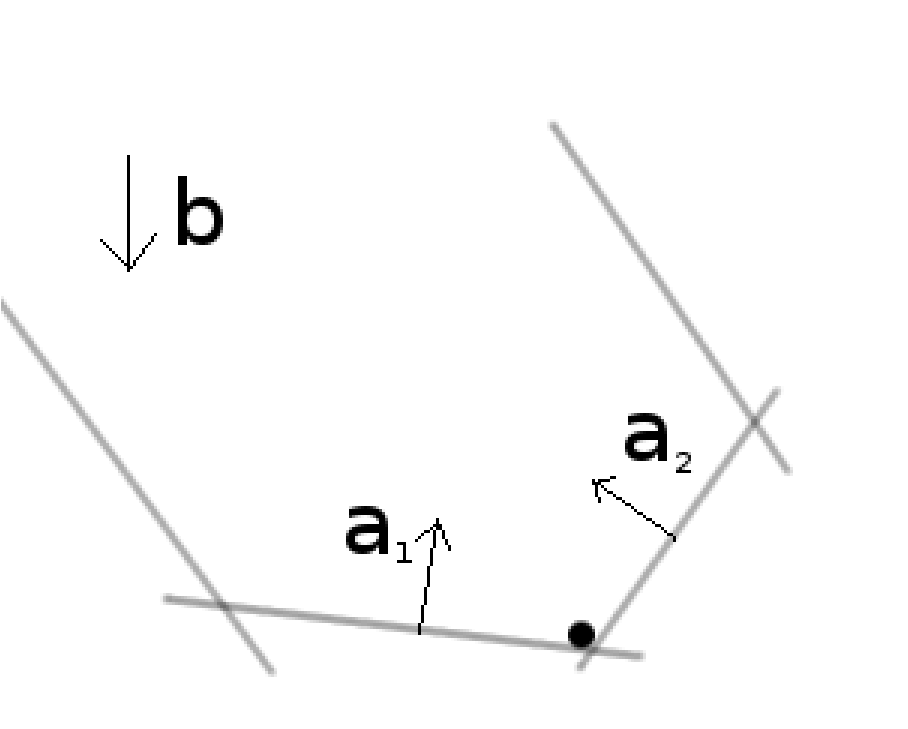
\includegraphics{gravity_ball.png}
  \label{fig:gravity-ball}
\end{center}
\end{figure}

The ball stopped because normal forces exerted by the walls cancel out the force of gravity. Denote the magnitude of the forces with $x_i$ and the directions in which they point with $a_i$. Then in order to cancel out gravity, we need: $\sum a_i x_i = b$. Also note that the forces always push, they don't pull, so $x_i \ge 0$.
Therefore, $x$ is feasible in the primal LP.

Note also that only the forces touching the ball can exert force, so if $y a_i \ge c_i$ then $x_i = 0$. This is equivalent to saying $(c_i - y a_i) x_i = 0$. Either $c_i = y a_i$ or $x_i = 0$.

Finally, we conclude that
$cx = \sum c_i x_i = \sum y a_i x_i = yAx = yb$.

The explanation why $\sum c_i x_i = \sum y a_i x_i$ is the following: either $c_i = y a_i$, in which case the terms on the two sides are equal, or $x_i=0$, in which case both terms, $y a_i x_i $ and $c_i x_i$, drop out from their respective sums.

\end{proof}

\end{document}
